\documentclass[11pt]{article}
\usepackage[margin=2cm,a4paper]{geometry}
\usepackage{graphicx}
\usepackage{float}
\usepackage{times}
\usepackage{array}
\usepackage{amsmath,amssymb,amsfonts,bm}
\usepackage{enumitem}
\usepackage{hyperref}
\usepackage{bookmark}
\usepackage[font=small,labelfont=bf,labelsep=none]{caption}
\usepackage[]{mdframed}
\usepackage{dsfont}
\usepackage{natbib}

\usepackage[T1]{fontenc}
\usepackage[utf8]{inputenc}
\usepackage{xcolor}
\usepackage{newtxmath}
% \numberwithin{equation}{section}

\usepackage{caption,subcaption}
\captionsetup[figure]{labelfont={bf},labelformat={default},labelsep=quad,name={Fig.}}
\captionsetup[table]{labelfont={bf},labelformat={default},labelsep=quad}
\captionsetup[subfigure]{labelfont={bf},labelformat=simple,labelsep=period}

\title{\vspace{-1em}Quasi-static elastic response to surface loading}
\date{\vspace{-3em}}

\begin{document}

\maketitle
\renewcommand{\baselinestretch}{1.25}

\section{Propagator matrix method}
\begin{large}
The propagator matrix method \citep{gilbert_1966, singh_1970} is applied to model the quasi-static elastic response to the surface loading. The subsurface elastic structure is idealized as a plane-layered medium over a uniform half-space. The method solves the static elasticity equilibrium equation and Hooke's law in the transform domain. The two horizontal directions are Fourier transformed to wavenumbers $k_x$ and $k_y$. Both the normal pressure and the horizontal shear traction at the surface are considered. In the transform domain, the elastic response decouples into the P-SV and SH systems, which are solved separately and superposed. For the P-SV system, the ordinary differential equation system is written as
\begin{equation}
    \frac{\mathrm{d}\mathbf{U}}{\mathrm{d}z} = \frac{\mathrm{d}}{\mathrm{d}z}
    \begin{bmatrix}
        U_1 \\ U_2 \\ U_3 \\ U_4
    \end{bmatrix} = \begin{bmatrix}
        0 & -k & \frac{1}{\mu} & 0 \\
        \frac{k\lambda}{\lambda+2\mu} & 0 & 0 & \frac{1}{\lambda+2\mu} \\
        \frac{4\mu k^2 (\lambda+\mu)}{\lambda+2\mu} & 0 & 0 & -\frac{k\lambda}{\lambda+2\mu} \\
        0 & 0 & k & 0
    \end{bmatrix} \begin{bmatrix}
        U_1 \\ U_2 \\ U_3 \\ U_4
    \end{bmatrix} = \mathbf{A}\mathbf{U}.
\label{elastic_ODE}
\end{equation}
The components of the displacement-stress vector $\mathbf{U}$ are defined as
\begin{equation}
\begin{aligned}
    -kU_1 &= ik_x \tilde{u}_x + ik_y \tilde{u}_y, \qquad & U_2 &= \tilde{u}_z, \\
    -kU_3 &= ik_x \tilde{\sigma}_{xz} + ik_y \tilde{\sigma}_{yz}, \qquad & U_4 &= \tilde{\sigma}_{zz},
\end{aligned}
\label{eq:def_psv}
\end{equation}
where $\Tilde{u}_i$ and $\Tilde{\sigma}_{ij}$ are displacement and stress components, respectively, in the Fourier domain under the following convention
\begin{equation}
    \Tilde{u}(k_x, k_y, z) = \int_{-\infty}^{+\infty} \int_{-\infty}^{+\infty} u(x,y,z)e^{-i(k_x x + k_y y)} \,\mathrm{d}x\mathrm{d}y,
\end{equation}
with horizontal wavenumbers $k_x$, $k_y$ and the magnitude $k = \sqrt{k_x^2 + k_y^2}$. For each elastic layer, the matrix $\mathbf{A}$ in Eq. (\ref{elastic_ODE}) is constructed from the Lam\'e parameters $\lambda$ and $\mu$ obtained from the density $\rho$ and P- and S-wave seismic velocities $v_P$ and $v_S$. We begin with the homogeneous solution at the top of the underlying half-space for each Fourier mode,
\begin{equation}
    \begin{bmatrix}
        U_1 \\ U_2 \\ U_3 \\ U_4
    \end{bmatrix} = c_1 \begin{bmatrix}
        \frac{1}{2k\mu} \\ \frac{1}{2k\mu} \\ 1 \\ 1
    \end{bmatrix} + c_2 \begin{bmatrix}
        \frac{\lambda+2\mu}{2k^2 \mu(\lambda+\mu)} \\ -\frac{1}{2k^2 (\lambda+\mu)} \\ \frac{1}{k} \\ 0
    \end{bmatrix},
\label{eq:initial}
\end{equation}
where $c_1(k_x, k_y)$ and $c_2(k_x,k_y)$ are coefficients to be determined by the surface conditions. This solution is then propagated upward through each layer by
\begin{equation}
    \mathbf{U}(z_{\text{top}}) = e^{\mathbf{A}h}\mathbf{U}(z_{\text{btm}}),
\end{equation}
where $z_{\text{top}}$ and $z_{\text{btm}}$ denote the top and bottom of the layer and $h = z_{\text{top}} - z_{\text{btm}}$ is the layer thickness. The propagator is the matrix exponential $e^{\mathbf{A}h}$. At the surface $z=0$, we impose the following boundary conditions
\begin{equation}
    U_3 = -\frac{ik_x \Tilde{t}_x + ik_y \Tilde{t}_y}{k},\qquad U_4 = -\Tilde{p}(k_x, k_y),\qquad \text{at}\,\,z=0
\label{eq:bc_psv}
\end{equation}
to solve for the coefficients $c_1$ and $c_2$, where $\Tilde{p}(k_x,k_y)$ and $\Tilde{t}_x(k_x,k_y)$, $\Tilde{t}_y(k_x,k_y)$ are the Fourier transforms of the input surface pressure and horizontal traction fields at a particular time. The in-plane component of the horizontal traction thus drives the P-SV system through $U_3$. Under the quasi-static assumption, we repeat solving for coefficients $c_1$ and $c_2$ given the surface loads at different times $t$. The final displacements and stress components are obtained from the inverse Fourier transform of $\mathbf{U}$ evaluated at the surface. The derivation can also be seen in \cite{segall_2010}.

The transverse component of the horizontal traction drives the SH system. Analogous to Eq. (\ref{eq:def_psv}), we define the displacement-stress vector $\mathbf{V}$ as
\begin{equation}
\begin{aligned}
    -kV_1 &= ik_x \tilde{u}_y - ik_y \tilde{u}_x, \qquad & -kV_2 &= ik_x \tilde{\sigma}_{yz} - ik_y \tilde{\sigma}_{xz},
\end{aligned}
\end{equation}
which satisfies the ordinary differential equation system
\begin{equation}
    \frac{\mathrm{d}\mathbf{V}}{\mathrm{d}z} = \frac{\mathrm{d}}{\mathrm{d}z}
    \begin{bmatrix}
        V_1 \\ V_2
    \end{bmatrix} = \begin{bmatrix}
        0 & \frac{1}{\mu} \\
        \mu k^2 & 0
    \end{bmatrix} \begin{bmatrix}
        V_1 \\ V_2
    \end{bmatrix} = \mathbf{B}\mathbf{V}.
\label{elastic_ODE_sh}
\end{equation}
The homogeneous solution at the top of the underlying half-space is
\begin{equation}
    \begin{bmatrix}
        V_1 \\ V_2
    \end{bmatrix} = c_3 \begin{bmatrix}
        \frac{1}{k\mu} \\ 1
    \end{bmatrix},
\label{eq:initial_sh}
\end{equation}
which is propagated upward through each layer by the propagator $e^{\mathbf{B}h}$, in the same way as the P-SV system. The coefficient $c_3(k_x,k_y)$ is determined by the surface boundary condition
\begin{equation}
    V_2 = -\frac{ik_x \Tilde{t}_y - ik_y \Tilde{t}_x}{k},\qquad \text{at}\,\,z=0.
\label{eq:bc_sh}
\end{equation}
The Cartesian components in the Fourier domain are recovered from the two systems by
\begin{equation}
\begin{aligned}
    \tilde{u}_x &= \frac{i}{k}\left(k_x U_1 - k_y V_1\right), \qquad & \tilde{u}_y &= \frac{i}{k}\left(k_y U_1 + k_x V_1\right), \\
    \tilde{\sigma}_{xz} &= \frac{i}{k}\left(k_x U_3 - k_y V_2\right), \qquad & \tilde{\sigma}_{yz} &= \frac{i}{k}\left(k_y U_3 + k_x V_2\right).
\end{aligned}
\label{eq:recover}
\end{equation}
Note that the SH system produces no vertical displacement and no dilatation, i.e. $\tilde{u}_z = \tilde{\sigma}_{zz} = 0$.

\end{large}

\section{Benchmark solutions}
\begin{large}
The Sorrells problem \citep{sorrells_1971} and Boussinesq problem \citep{boussinesq_1885} are used to benchmark the propagator matrix method for surface pressure loading (Fig. \ref{fig:halfspace}). For horizontal traction loading, the corresponding benchmarks are the Cerruti problem \citep{cerruti_1882} and a Sorrells-type problem under a shear traction wave, both of which exercise the P-SV and SH systems simultaneously. As we solve the elasticity equation in the Fourier domain, periodic loading is exactly represented, and the Sorrells-type problems are well-suited to this method. On the other hand, for the Boussinesq and Cerruti problems, the domain-averaged mean of the analytical solution should be removed to compare with the numerical result. We can notice from Eq. (\ref{eq:initial}) that the zero-wavenumber component ($k=0$) needs to be separately considered since $k$ appears in the denominator of the initial homogeneous solution. This component is not included in the solution.

\end{large}

\begin{figure}[!h]
    \centering
    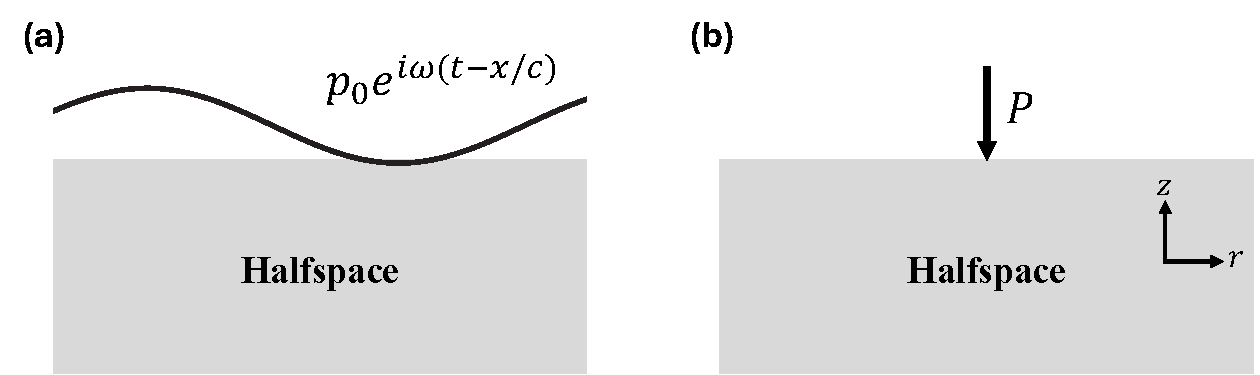
\includegraphics[width=0.75\linewidth]{Figures/Halfspace.pdf}
    \caption{The configuration of benchmark problems. \textbf{(a)} Sorrells problem. The elastic halfspace is subject to a monochromatic pressure wave loading with phase speed $c$ much smaller than the elastic wave speed. \textbf{(b)} Boussinesq problem. The elastic halfspace is subject to a concentrated normal load $P$. The cylindrical coordinates are defined with the positive $z$-axis pointing upward.}
    \label{fig:halfspace}
\end{figure}

\subsection{Sorrells problem}
\begin{large}
With the quasi-static assumption $c \ll v_{P,S}$ and $\omega z c\ll 2v_{P,S}^2$, the displacement field of the Sorrells problem is given as
\begin{align}
    u_x &= \frac{icp_0}{2\mu\omega}\left(\frac{v_S^2}{v_P^2 - v_S^2} - \frac{\omega |z|}{c}\right) e^{-\omega|z|/c}\, e^{i\omega (t-x/c)}, \nonumber \\
    u_z &= -\frac{cp_0}{2\mu\omega}\left(\frac{v_P^2}{v_P^2 - v_S^2} + \frac{\omega |z|}{c}\right) e^{-\omega|z|/c}\, e^{i\omega (t-x/c)}.
\label{eq:Sorrells}
\end{align}
Eq. (\ref{eq:Sorrells}) shows an exponential decay in $z$-direction, and in fact it only depends on the wavenumber $k=\omega /c$. At the surface $z=0$, the displacement amplitude ratio is $|u_x/u_z| = (v_S/v_P)^2$, which is much smaller than 1 for compliant sediments. The comparison of analytical and numerical results is shown in Fig. \ref{fig:Sorrells}

\end{large}

\begin{figure}[!t]
    \centering
    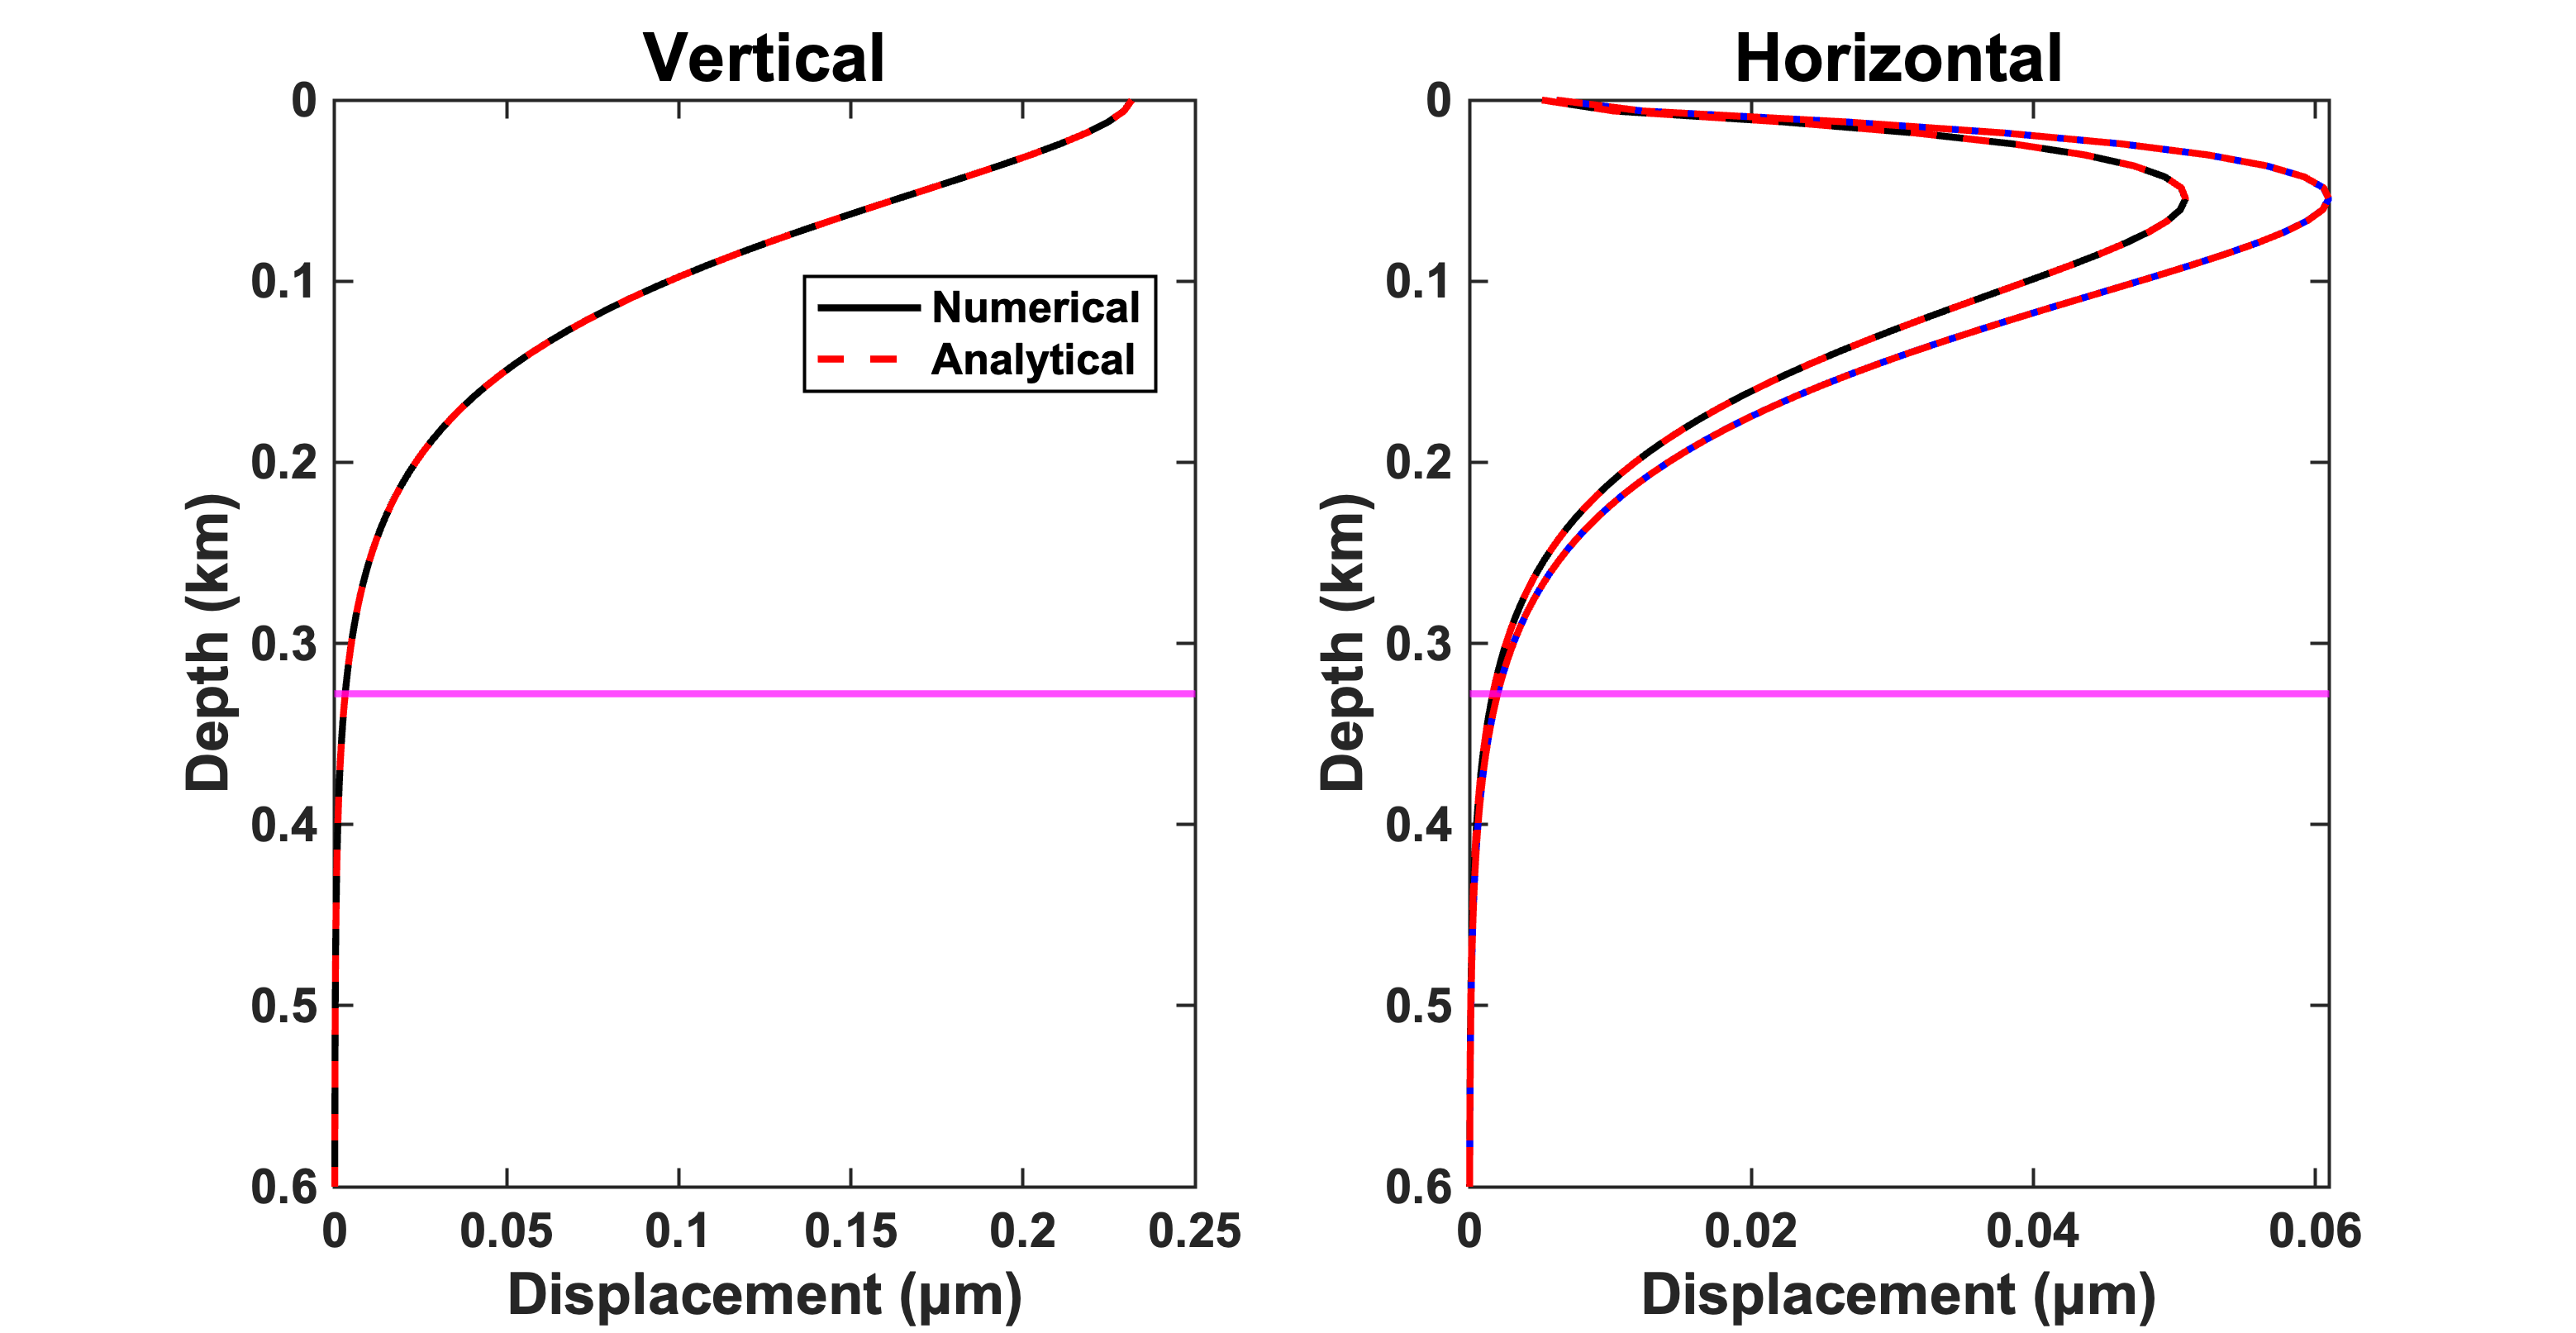
\includegraphics[width=0.85\linewidth]{Figures/Sorrells.png}
    \caption{Benchmark of Sorrells problem with $p_0 = 1$ Pa, $\lambda = 0.328$ km and wave azimuth $\theta = 50^{\circ}$. The magenta line indicates the depth $|z|=\lambda$ as a reference to indicate the exponential decay rate.}
    \label{fig:Sorrells}
\end{figure}

\subsection{Boussinesq problem}
\begin{large}
The Boussinesq solution describes the static elastic response of a homogeneous half-space subject to a concentrated normal load $P$. This is the first benchmark for the propagator matrix method. In the polar coordinate, we have $u_\theta = 0$ and
\begin{align}
    u_r &= \frac{Pr}{4\pi\mu} \left[\frac{|z|}{R^3} - \frac{1-2\nu}{R(|z|+R)}\right],\nonumber\\
    u_z &= -\frac{P}{4\pi\mu} \left[\frac{2(1-\nu)}{R} + \frac{|z|^2}{R^3}\right],
\label{eq:displ}
\end{align}
where $r = \sqrt{x^2 + y^2}$ and $R = \sqrt{r^2 + z^2}$ \citep{slaughter_2002}. Here, the solution is written in terms of $|z|$, the depth from the surface. For the stress components, we have $\sigma_{r\theta} = \sigma_{\theta z} = 0$ and
\begin{align}
    \sigma_{rr} &= \frac{P}{2\pi} \left[\frac{1-2\nu}{R(|z|+R)} - \frac{3r^2 |z|}{R^5}\right], \nonumber \\
    \sigma_{\theta\theta} &= \frac{P(1-2\nu)}{2\pi} \left[\frac{|z|}{R^3} - \frac{1}{R(|z|+R)}\right], \nonumber \\
    \sigma_{zz} &= -\frac{3P|z|^3}{2\pi R^5}, \qquad \sigma_{rz} = \frac{3Pr|z|^2}{2\pi R^5}.
\label{eq:stress}
\end{align}
The comparison of analytical and numerical results is shown in Fig. \ref{fig:Boussinesq}.

\end{large}

\begin{figure}[!t]
    \centering
    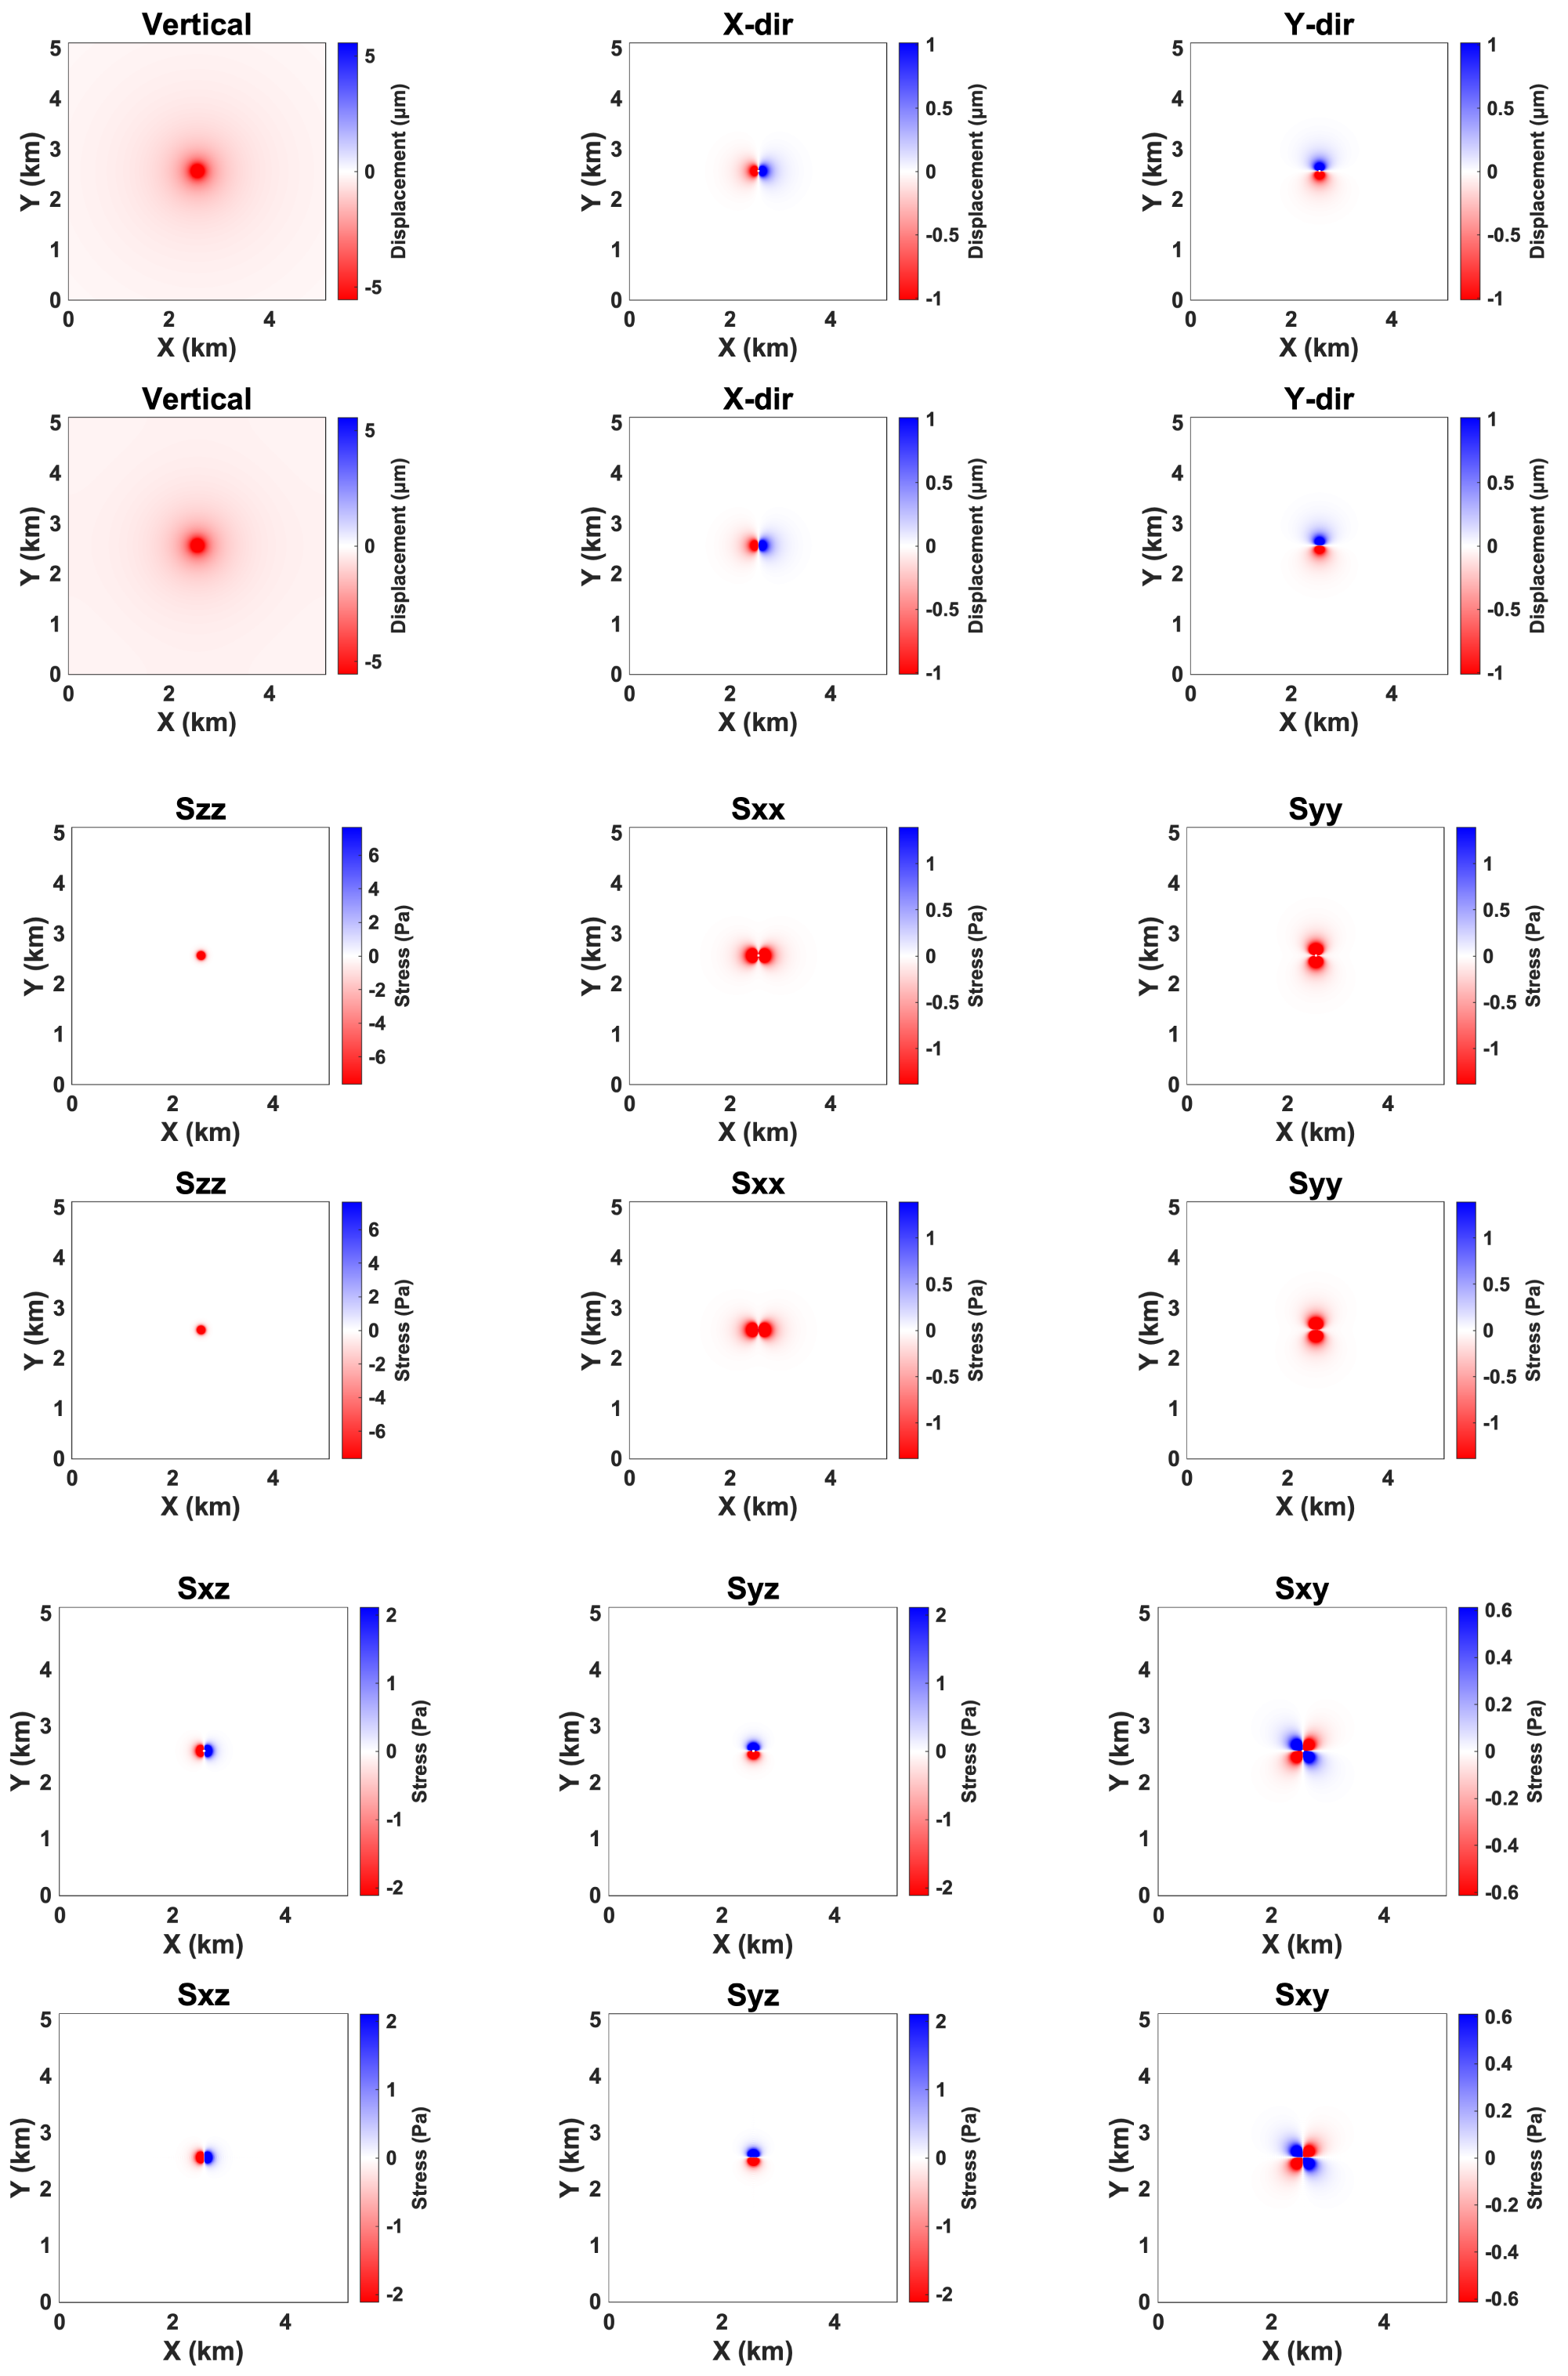
\includegraphics[width=0.85\linewidth]{Figures/Boussinesq.png}
    \caption{Benchmark of Boussinesq problem with $P = 10^6$ N at depth $z = 0.05$ km. The properties of the elastic halfspace are $\rho = 1600$ kg$/$m$^3$, $v_P = 1.45$ km$/$s and $v_S = 0.27$ km$/$s. The analytical solutions from Eqs (\ref{eq:displ}) and (\ref{eq:stress}) are plotted on the top, while the numerical solutions are plotted on the bottom for each displacement and stress component.}
    \label{fig:Boussinesq}
\end{figure}

\subsection{Sorrells problem under shear traction}
\begin{large}
The analog of the Sorrells problem for horizontal traction loading considers a shear traction wave $\tau_0 e^{i\omega(t-x/c)}$ applied at the surface of the elastic halfspace. When the traction is applied along the direction of propagation $x$ (in-plane), only the P-SV system is excited, and the static solution is
\begin{align}
    u_x &= \frac{c\tau_0}{2\mu\omega}\left(\frac{v_P^2}{v_P^2 - v_S^2} - \frac{\omega |z|}{c}\right) e^{-\omega|z|/c}\, e^{i\omega (t-x/c)}, \nonumber \\
    u_z &= -\frac{ic\tau_0}{2\mu\omega}\left(\frac{v_S^2}{v_P^2 - v_S^2} + \frac{\omega |z|}{c}\right) e^{-\omega|z|/c}\, e^{i\omega (t-x/c)},
\label{eq:Sorrells_shear}
\end{align}
which mirrors Eq. (\ref{eq:Sorrells}): at the surface $z=0$, the displacement amplitude ratio is $|u_z/u_x| = (v_S/v_P)^2$. When the traction is applied transverse to the direction of propagation (along $y$), only the SH system is excited, and the static solution is
\begin{equation}
    u_y = \frac{c\tau_0}{\mu\omega}\, e^{-\omega|z|/c}\, e^{i\omega (t-x/c)}.
\label{eq:Sorrells_sh}
\end{equation}
For a general traction azimuth, the traction is decomposed into the in-plane and transverse components, and the two responses are superposed. Note from Eqs (\ref{eq:Sorrells_shear}) and (\ref{eq:Sorrells_sh}) that the in-plane and transverse horizontal displacements are in phase with the traction wave, while the vertical displacement is shifted by $90^{\circ}$. The comparison of analytical and numerical results is shown in Fig. \ref{fig:Sorrells_shear}, where the traction is applied along $x$ while the wave propagates at an azimuth of $50^{\circ}$, so that both the P-SV and SH systems contribute.

\end{large}

\begin{figure}[!t]
    \centering
    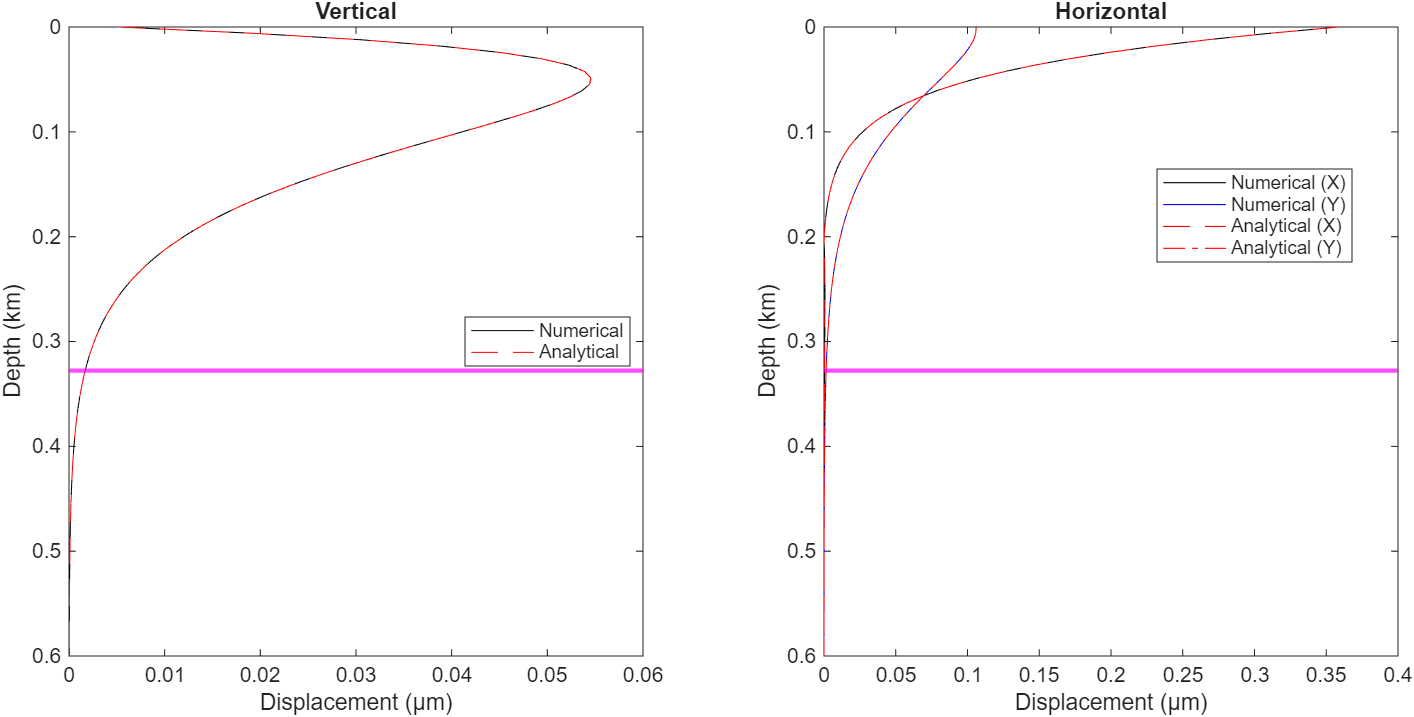
\includegraphics[width=0.85\linewidth]{Figures/Sorrells_shear.png}
    \caption{Benchmark of Sorrells problem under shear traction with $\tau_0 = 1$ Pa, $\lambda = 0.328$ km, wave azimuth $\theta = 50^{\circ}$ and traction along the $x$-axis. The magenta line indicates the depth $|z|=\lambda$ as a reference to indicate the exponential decay rate.}
    \label{fig:Sorrells_shear}
\end{figure}

\subsection{Cerruti problem}
\begin{large}
The Cerruti solution \citep{cerruti_1882} describes the static elastic response of a homogeneous half-space subject to a concentrated horizontal load $Q$, taken here along the $+x$ direction. It is the counterpart of the Boussinesq problem for horizontal traction loading, and provides a benchmark in which the P-SV and SH systems are excited simultaneously. The displacement field is given as
\begin{align}
    u_x &= \frac{Q}{4\pi\mu} \left[\frac{1}{R} + \frac{x^2}{R^3} + (1-2\nu)\left(\frac{1}{R+|z|} - \frac{x^2}{R(R+|z|)^2}\right)\right],\nonumber\\
    u_y &= \frac{Qxy}{4\pi\mu} \left[\frac{1}{R^3} - \frac{1-2\nu}{R(R+|z|)^2}\right],\nonumber\\
    u_z &= -\frac{Qx}{4\pi\mu} \left[\frac{|z|}{R^3} + \frac{1-2\nu}{R(R+|z|)}\right],
\label{eq:displ_cerruti}
\end{align}
written in terms of the depth $|z|$ with the positive $z$-axis pointing upward \citep{slaughter_2002}. The stress components are derived from Eq. (\ref{eq:displ_cerruti}) with Hooke's law (and verified symbolically against the equilibrium equation and the traction-free surface condition),
\begin{align}
    \sigma_{xx} &= \frac{Qx}{2\pi R^3} \left[-\frac{3x^2}{R^2} + \frac{1-2\nu}{(R+|z|)^2}\left(R^2 - y^2 - \frac{2Ry^2}{R+|z|}\right)\right], \nonumber \\
    \sigma_{yy} &= \frac{Qx}{2\pi R^3} \left[-\frac{3y^2}{R^2} + \frac{1-2\nu}{(R+|z|)^2}\left(3R^2 - x^2 - \frac{2Rx^2}{R+|z|}\right)\right], \nonumber \\
    \sigma_{xy} &= \frac{Qy}{2\pi R^3} \left[-\frac{3x^2}{R^2} + \frac{1-2\nu}{(R+|z|)^2}\left(-R^2 + x^2 + \frac{2Rx^2}{R+|z|}\right)\right], \nonumber \\
    \sigma_{zz} &= -\frac{3Qx|z|^2}{2\pi R^5}, \qquad \sigma_{xz} = \frac{3Qx^2|z|}{2\pi R^5}, \qquad \sigma_{yz} = \frac{3Qxy|z|}{2\pi R^5}.
\label{eq:stress_cerruti}
\end{align}
The comparison of analytical and numerical results is shown in Figs \ref{fig:Cerruti_disp} and \ref{fig:Cerruti_stress}.

\end{large}

\begin{figure}[!t]
    \centering
    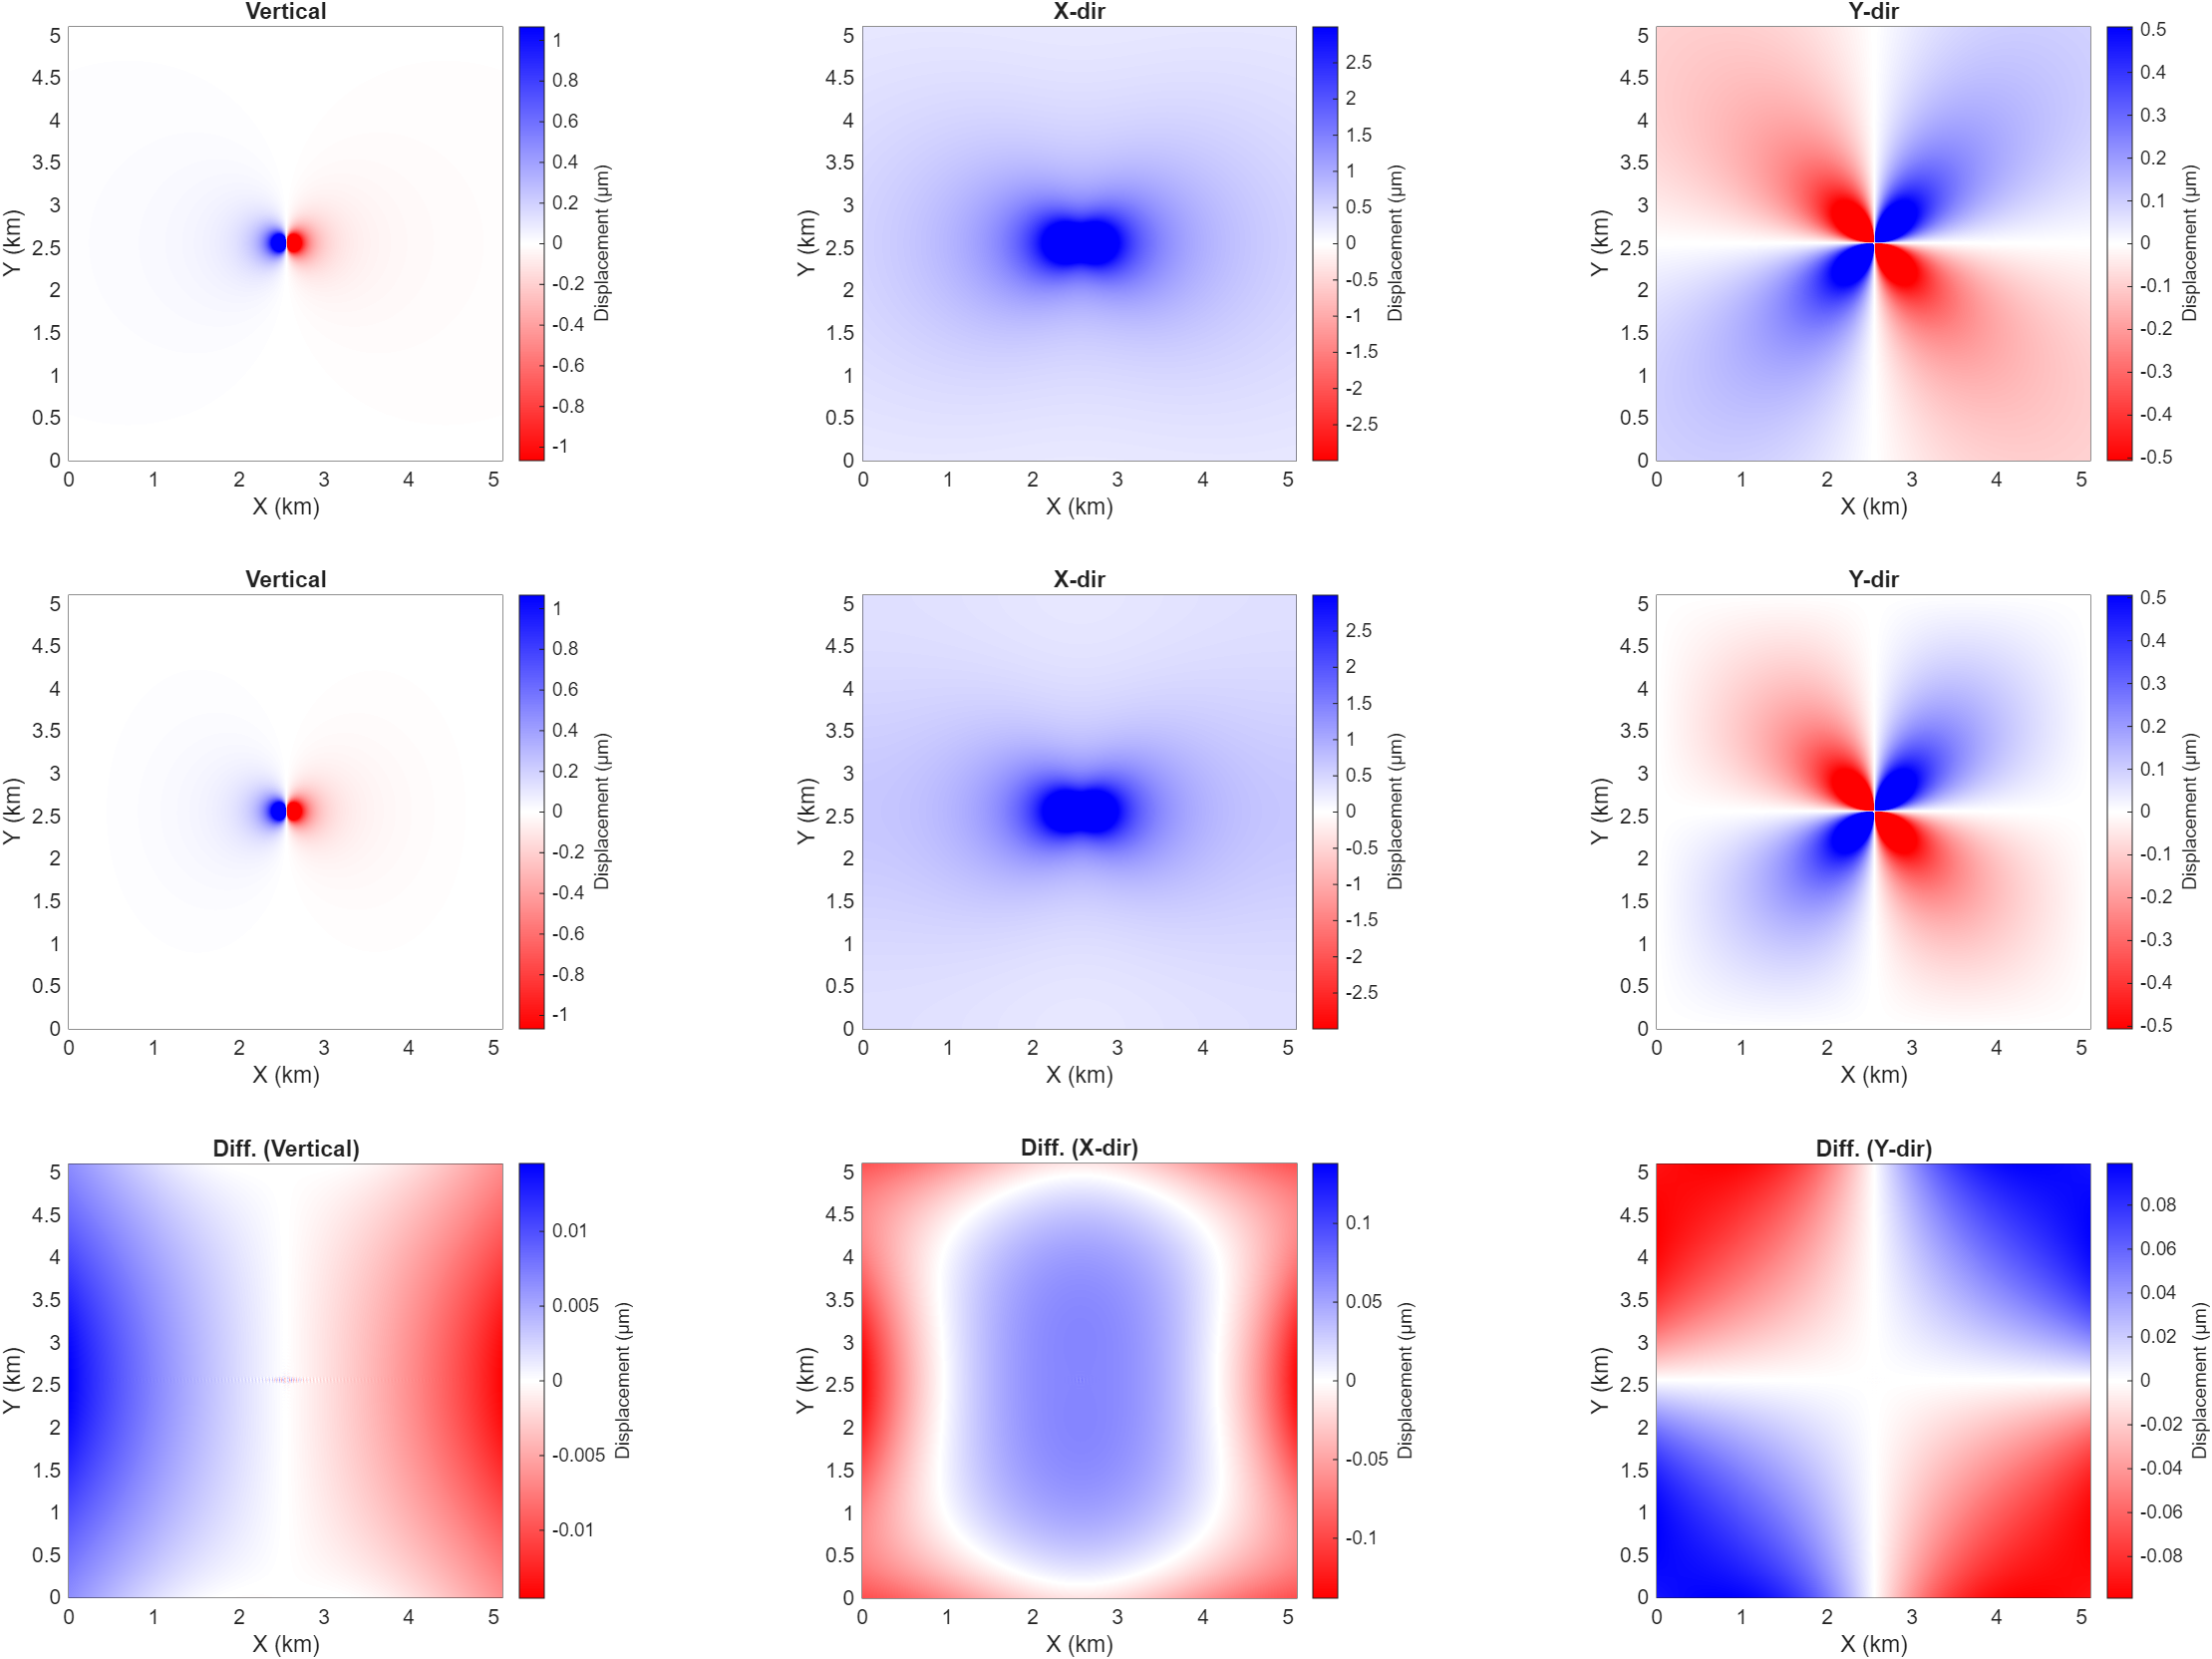
\includegraphics[width=0.85\linewidth]{Figures/Cerruti_disp.png}
    \caption{Benchmark of Cerruti problem: displacement components with $Q = 10^6$ N along $+x$ at depth $z = 0.05$ km. The properties of the elastic halfspace are the same as in Fig. \ref{fig:Boussinesq}. The analytical solutions from Eq. (\ref{eq:displ_cerruti}) are plotted on the top, the numerical solutions in the middle, and their differences on the bottom.}
    \label{fig:Cerruti_disp}
\end{figure}

\begin{figure}[!t]
    \centering
    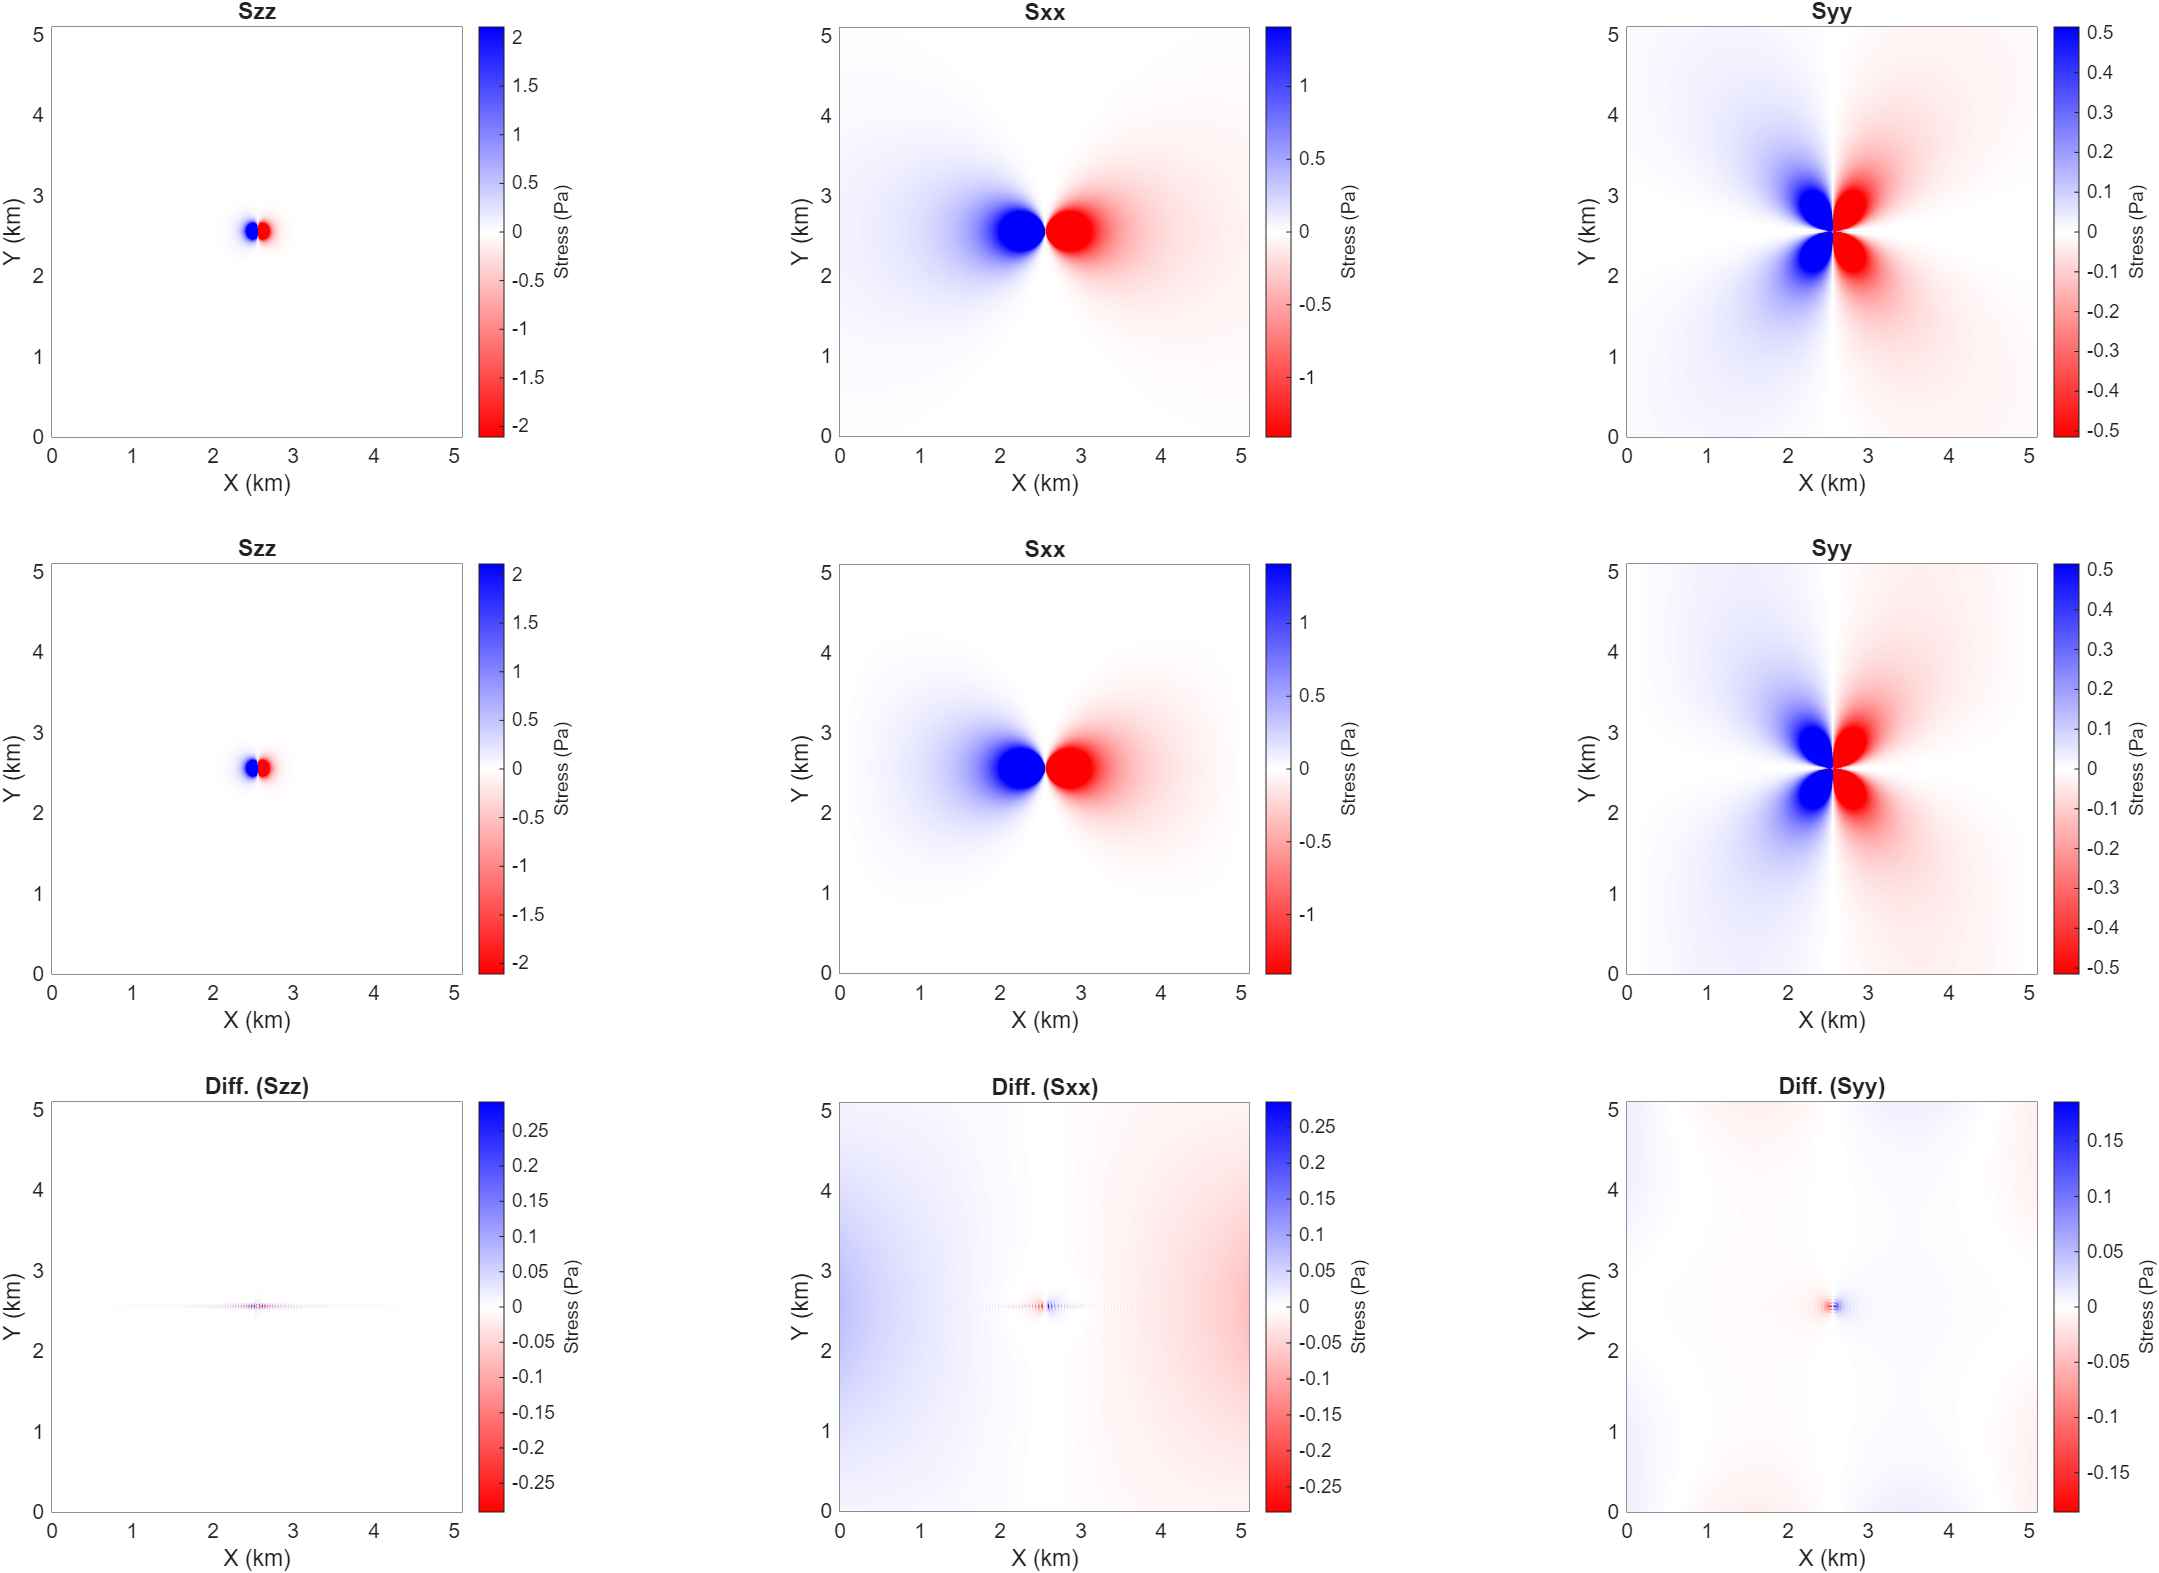
\includegraphics[width=0.75\linewidth]{Figures/Cerruti_normal_stress.png}
    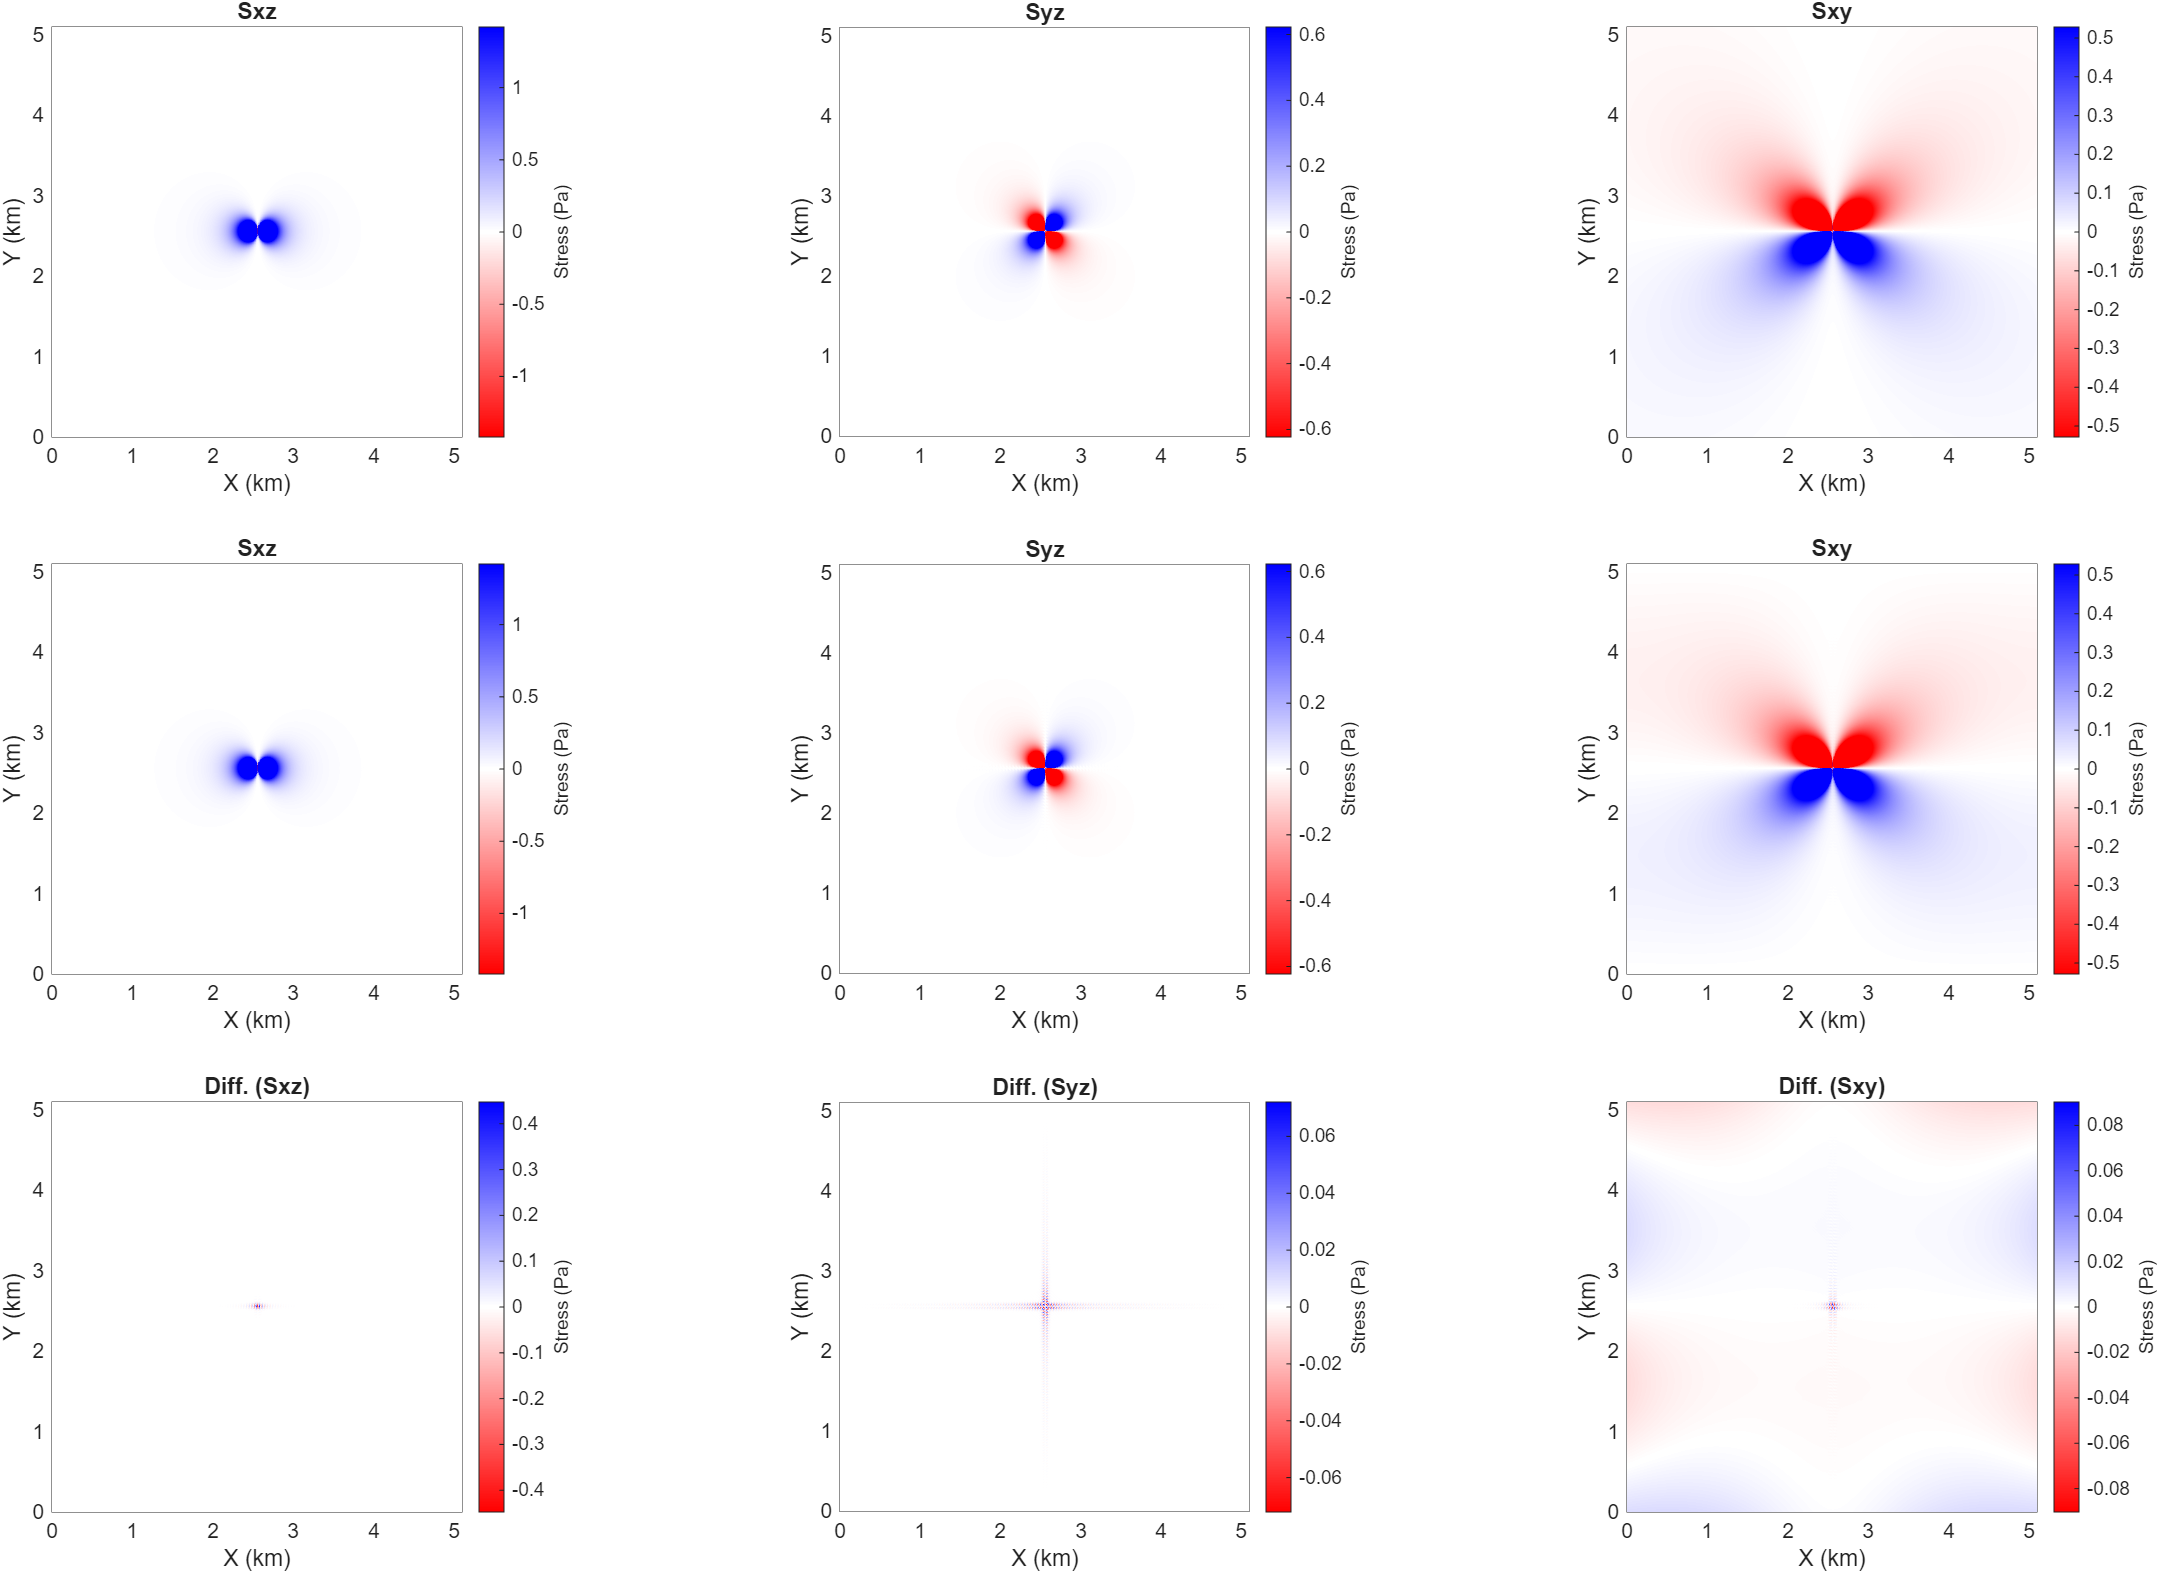
\includegraphics[width=0.75\linewidth]{Figures/Cerruti_shear_stress.png}
    \caption{Benchmark of Cerruti problem: normal (top panel) and shear (bottom panel) stress components, with the same configuration as Fig. \ref{fig:Cerruti_disp}. Within each panel, the analytical solutions from Eq. (\ref{eq:stress_cerruti}) are plotted on the top, the numerical solutions in the middle, and their differences on the bottom.}
    \label{fig:Cerruti_stress}
\end{figure}

\clearpage
\bibliography{refs}
\bibliographystyle{apalike}

\end{document}